\documentclass[10pt,xcolor=svgnames]{beamer} %Beamer

\usepackage{palatino} %font type
\usepackage{xcolor}
\usepackage[font={small}]{caption}
\usefonttheme{metropolis} %Type of slides
\usefonttheme[onlymath]{serif} %font type Mathematical expressions
\usetheme[progressbar=frametitle,titleformat frame=smallcaps,numbering=counter]{metropolis} %This adds a bar at the beginning of each section.
\useoutertheme[subsection=false]{miniframes} %Circles in the top of each frame, showing the slide of each section you are at



\usepackage{appendixnumberbeamer} %enumerate each slide without counting the appendix

\definecolor{SysBlue}{RGB}{0,0,0}
\definecolor{Progress}{RGB}{56,60,92}
\definecolor{Header}{RGB}{25,25,25}
\definecolor{SlideTitle}{RGB}{0,0,0}
\definecolor{ToC}{RGB}{51,58,66}

\setbeamercolor{progress bar}{fg=Progress} %These are the colours of the progress bar. Notice that the names used are the svgnames
\setbeamercolor{title separator}{fg=SysBlue} %This is the line colour in the title slide
\setbeamercolor{structure}{fg=black} %Colour of the text of structure, numbers, items, blah. Not the big text.
\setbeamercolor{normal text}{fg=black!87} %Colour of normal text
\setbeamercolor{alerted text}{fg=DarkRed!60!Gainsboro} %Color of the alert box
\setbeamercolor{example text}{fg=ToC} %Colour of the Example block text
\setbeamercolor{background canvas}{bg=white}


\setbeamercolor{palette primary}{bg=SlideTitle, fg=white} %These are the colours of the background. Being this the main combination and so one. 
\setbeamercolor{palette secondary}{bg=Header, fg=white}
\setbeamercolor{palette tertiary}{bg=Header, fg=white}
\setbeamercolor{section in toc}{fg=ToC} %Color of the text in the table of contents (toc)

\setbeamertemplate{caption}{\raggedright\insertcaption\par}
\setbeamertemplate{frame numbering}[none]
\setbeamertemplate{blocks}[rounded][shadow=true]


%These next packages are the useful for Physics in general, you can add the extras here. 
\usepackage{amsmath,amssymb}
\usepackage{slashed}
\usepackage{cite}
\usepackage{relsize}
\usepackage{caption}
\usepackage{subcaption}
\usepackage{multicol}
\usepackage{booktabs}
\usepackage[scale=2]{ccicons}
\usepackage{pgfplots}
\usepgfplotslibrary{dateplot}
\usepackage{geometry}
\usepackage{xspace}

\usepackage{textpos} 

\newcommand{\red}[1]{\textcolor{red}{#1}}

\addtobeamertemplate{frametitle}{}{%
    \begin{textblock*}{200mm}(.85\textwidth,-0.85cm)
        
\includegraphics[height=0.55cm,width=2.5cm]{logo_header}
    \end{textblock*}}

\newcommand{\themename}{\textbf{\textsc{bluetemp}\xspace}}%metropolis}}\xspace}

\title{Pachira Fund}
\author[Name]{Ian Moore, PhD \inst{$\dagger$}}%With inst, you can change the institution they belong
\subtitle{Can Money Grow on Trees?}

\institute[shortinst]{\inst{$\dagger$} Tokenomics Researcher / Engineer @ Syslabs (email: imoore@syscoin.org) }

\date{November 13, 2023} %Here you can change the date
\titlegraphic{\vspace{-0.5cm}\hfill
\includegraphics[scale=0.23]{logo.png}} %You can modify the location of the logo by changing the command \vspace{}. 

\begin{document}
{

\setbeamercolor{background canvas}{bg=white, fg=black}
\setbeamercolor{normal text}{fg=black}
}%This is the colour of the first slide. bg= background and fg=foreground

\metroset{sectionpage=none} 

\section{Problem}

\begin{frame}{Stagnant Liquidity Problem} 

\metroset{block=fill}
\begin{exampleblock}{\textsc{Problem:}}
\begin{itemize}
  \item How do we increase trading volume on stagnated liquidity in pool over some time interval $t$?
\end{itemize}
\end{exampleblock}

\begin{figure}[h!]
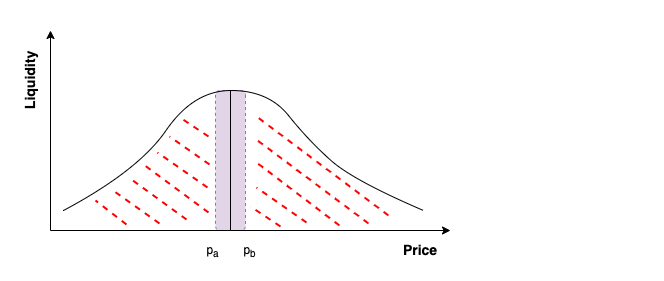
\includegraphics[width=3.5in]{img/freq0.png}
\caption{ Liquidity Frequency Distribution} 
\label{fig:full_tree}
\end{figure}

\end{frame}



\begin{frame}{Stagnant Liquidity Problem} 

\metroset{block=fill}
\begin{exampleblock}{\textsc{Problem:}}
\begin{itemize}
  \item How do we increase trading volume on stagnated liquidity in pool over some time interval $t$?
\end{itemize}
\end{exampleblock}

\begin{figure}[h!]
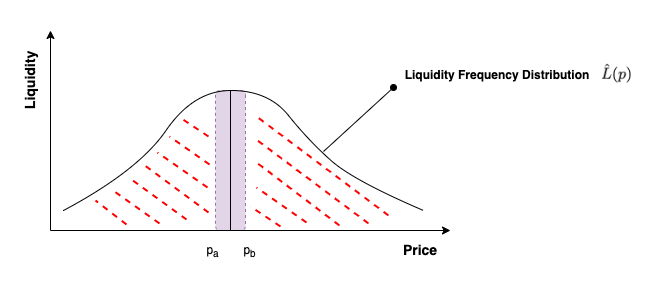
\includegraphics[width=3.5in]{img/freq1.png}
\caption{ Liquidity Frequency Distribution} 
\label{fig:full_tree}
\end{figure}

\end{frame}


\begin{frame}{Stagnant Liquidity Problem} 

\metroset{block=fill}
\begin{exampleblock}{\textsc{Problem:}}
\begin{itemize}
  \item How do we increase trading volume on stagnated liquidity in pool over some time interval $t$?
\end{itemize}
\end{exampleblock}

\begin{figure}[h!]
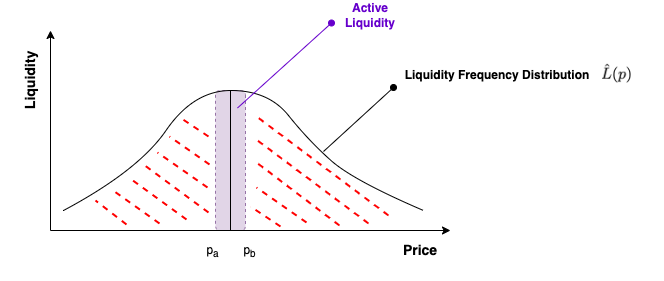
\includegraphics[width=3.5in]{img/freq2.png}
\caption{ Liquidity Frequency Distribution} 
\label{fig:full_tree}
\end{figure}

\end{frame}


\begin{frame}{Stagnant Liquidity Problem} 

\metroset{block=fill}
\begin{exampleblock}{\textsc{Problem:}}
\begin{itemize}
  \item How do we increase trading volume on stagnated liquidity in pool over some time interval $t$?
\end{itemize}
\end{exampleblock}

\begin{figure}[h!]
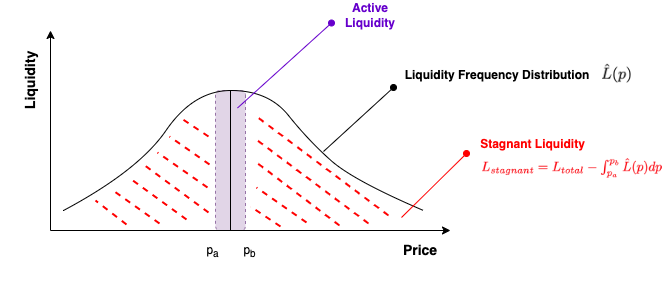
\includegraphics[width=3.5in]{img/freq3.png}
\caption{ Liquidity Frequency Distribution} 
\label{fig:full_tree}
\end{figure}

\end{frame}



\begin{frame}{Stagnant Liquidity Problem} 

\metroset{block=fill}
\begin{exampleblock}{\textsc{Problem:}}
\begin{itemize}
  \item How do we increase trading volume on stagnated liquidity in pool over some time interval $t$?
\end{itemize}
\end{exampleblock}

\begin{figure}[h!]
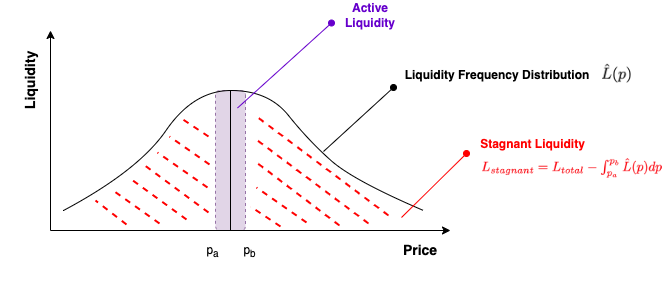
\includegraphics[width=3.5in]{img/freq3.png}
\caption{ Liquidity Frequency Distribution} 
\label{fig:full_tree}
\end{figure}

\begin{exampleblock}{}
We call this inefficiency the \red{Stagnant Liquidity Problem}
\end{exampleblock}

\end{frame}

\section{Liquidity Trees}

\begin{frame}{Solution: Liquidity Trees} 

\metroset{block=fill}
\begin{exampleblock}{\textsc{Solution}}
\begin{itemize}
  \item Instead of adjusting the price curve as individual LPs
\end{itemize}
\end{exampleblock}

\vspace{7cm}

\end{frame}


\begin{frame}{Solution: Liquidity Trees} 

\metroset{block=fill}
\begin{exampleblock}{\textsc{Solution}}
\begin{itemize}
  \item Instead of adjusting the price curve as individual LPs, we address the problem via a \red{system} of LPs called \red{Liquidity Trees}
\end{itemize}
\end{exampleblock}

\vspace{7cm}

\end{frame}

\begin{frame}{Solution: Liquidity Trees} 

\metroset{block=fill}
\begin{exampleblock}{\textsc{Solution}}
\begin{itemize}
  \item Instead of adjusting the price curve as individual LPs, we address the problem via a \red{system} of LPs called \red{Liquidity Trees}
\end{itemize}
\end{exampleblock}

\begin{figure}[h!]
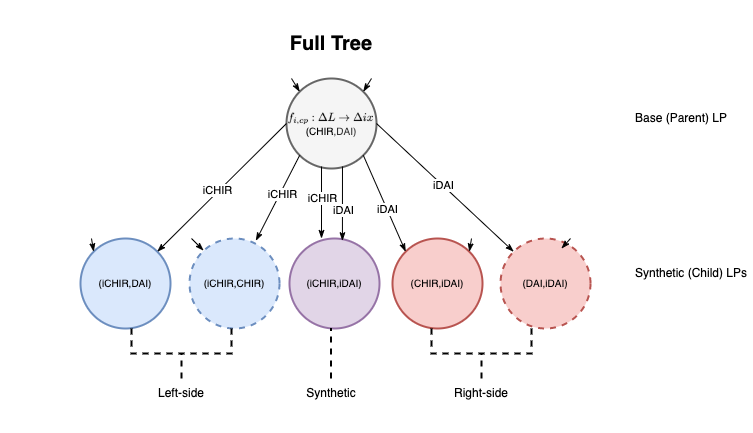
\includegraphics[width=3in]{img/full_tree.png}
\caption{Full CPT liquidity tree represented as a computational tree structure comprised of left-sided, right-sided and synthetic pools } 
\label{fig:full_tree}
\end{figure}

\end{frame}




\section{ETHDenver 2024}

\begin{frame}{Summary}

\metroset{block=fill}
\begin{exampleblock}{\textsc{ETHDenver 2024:}}
\begin{itemize}
  \item Defining the stagnant liquidity problem
  \item Addressing the problem using a new DeFi primitive, which we call Liquidity Trees 
  \item Show simulations to support our reasoning
  \item Discuss how we will be integrating Liquidity Trees for the Pachira token launch (\$CHIR)
\end{itemize}
\end{exampleblock}
\end{frame}


\end{document}